\documentclass[12pt]{article}
\usepackage{amsmath}
\usepackage{graphicx}
\usepackage{hyperref}
\usepackage{listings}
\usepackage{color}
\usepackage{pythonhighlight}

\title{Operating System Course Report - First Half of the Semester}
\author{A class}
\date{\today}

\begin{document}

\maketitle
\newpage

\tableofcontents
\newpage

\section{Introduction}
This report summarizes the topics covered during the first half of the Operating System course. It includes theoretical concepts, practical implementations, and assignments. The course focuses on the fundamentals of operating systems, including system architecture, process management, CPU scheduling, and deadlock handling.

\section{Course Overview}
\subsection{Objectives}
The main objectives of this course are:
\begin{itemize}
    \item To understand the basic components and architecture of a computer system.
    \item To learn process management, scheduling, and inter-process communication.
    \item To explore file systems, input/output management, and virtualization.
    \item To study the prevention and handling of deadlocks in operating systems.
\end{itemize}

\subsection{Course Structure}
The course is divided into two halves. This report focuses on the first half, which covers:
\begin{itemize}
    \item Basic Concepts and Components of Computer Systems
    \item System Performance and Metrics
    \item System Architecture of Computer Systems
    \item Process Description and Control
    \item Scheduling Algorithms
    \item Process Creation and Termination
    \item Introduction to Threads
    \item File Systems
    \item Input and Output Management
    \item Deadlock Introduction and Prevention
    \item User Interface Management
    \item Virtualization in Operating Systems
\end{itemize}

\section{Topics Covered}

\subsection{Basic Concepts and Components of Computer Systems}
This section explains the fundamental components that make up a computer system, including the CPU, memory, storage, and input/output devices.

\subsection{System Performance and Metrics}
This section introduces various system performance metrics used to measure the efficiency of a computer system, including throughput, response time, and utilization.

\subsection{System Architecture of Computer Systems}
Describes the architecture of modern computer systems, focusing on the interaction between hardware and the operating system.

\subsection{Process Description and Control}
Processes are a central concept in operating systems. This section covers:
\begin{itemize}
    \item Process states and state transitions
    \item Process control block (PCB)
    \item Context switching
\end{itemize}

\subsection{Scheduling Algorithms}
This section covers:
\begin{itemize}
    \item First-Come, First-Served (FCFS)
    \item Shortest Job Next (SJN)
    \item Round Robin (RR)
\end{itemize}
It explains how these algorithms are used to allocate CPU time to processes.

\subsection{Process Creation and Termination}
Details how processes are created and terminated by the operating system, including:
\begin{itemize}
    \item Process spawning
    \item Process termination conditions
\end{itemize}

\subsection{Introduction to Threads}
This section introduces the concept of threads and their relation to processes, covering:
\begin{itemize}
    \item Single-threaded vs. multi-threaded processes
    \item Benefits of multithreading
\end{itemize}

\begin{figure}[h]
    \centering
    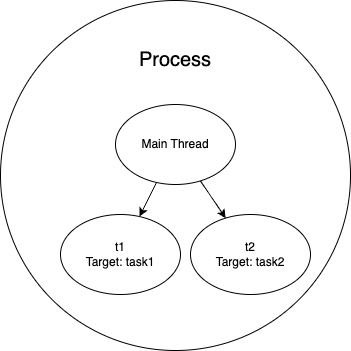
\includegraphics[width=0.5\textwidth]{/Users/khawaritzmi/Unhas/os_report_mid2024/a_class/asset/example.png}  % Sesuaikan nama file dan ukurannya
    \caption{Ini adalah gambar contoh dari multithreading.}
    \label{fig:contoh_gambar}
\end{figure}

Seperti yang terlihat pada Gambar \ref{fig:contoh_gambar}, inilah cara menambahkan gambar dengan keterangan.

\subsection{File Systems}
File systems provide a way for the operating system to store, retrieve, and manage data. This section explains:
\begin{itemize}
    \item File system structure
    \item File access methods
    \item Directory management
\end{itemize}

\subsection{Input and Output Management}
Input and output management is key for handling the interaction between the system and external devices. This section includes:
\begin{itemize}
    \item Device drivers
    \item I/O scheduling
\end{itemize}

\subsection{Deadlock Introduction and Prevention}
Explores the concept of deadlocks and methods for preventing them:
\begin{itemize}
    \item Deadlock conditions
    \item Deadlock prevention techniques
    \item Resource Allocation Denial
        
    \hspace{1cm} Sistem operasi menganalisis permintaan sumber daya dari proses secara saksama dan menentukan  apakah pemberian sumber daya tertentu akan menyebabkan kondisi \textit{unsafe} atau potensi \textit{deadlock}. Jika pemberian sumber daya dianggap tidak aman, sistem akan menolak permintaan sumber daya untuk menghindari \textit{deadlock}. 
        
    \hspace{1cm}Salah satu contoh kasus dengan metode ini adalah ketika proses P1 meminta sumber daya R1. Sebelum mengalokasikan sumber daya, sistem mengevaluasi apakah proses lain bisa menyelesaikan eksekusi dengan sumber daya yang tersisa.Jika tidak, permintaan P1 ditolak sementara waktu dan akan dilanjutkan ketika semua sumber daya yang dibutuhkan sudah lengkap.
    
    \item Reource Ordering

    \hspace{1cm} Sistem operasi menetapkan pengenal numerik yang unik untuk setiap sumber daya dan memastikan bahwa proses hanya dapat meminta sumber daya dalam urutan yang meningkat. Hal ini memastikan bahwa proses tidak pernah memasuki status \textit{circular wait} dan mencegah \textit{deadlock}.
    
    \hspace{1cm} Salah satu contoh kasusnya saat sumber daya 1 harus selalu diminta sebelum sumber daya 2 jika Proses 1 ingin meminta kedua sumber daya. Karena sistem menetapkan urutan, proses 1 harus meminta Sumber daya 1 terlebih dahulu. Jika mendapatkannya, baru boleh meminta sumber daya 2.

    \item Avoidance of Hold-and-wait conditions

    \hspace{1cm} Proses harus meminta semua sumber daya yang dibutuhkan di awal (sebelum memulai eksekusi) atau melepaskan sumber daya yang sedang dipegang sebelum meminta sumber daya tambahan, sehingga menghilangkan kemungkinan \textit{hold and wait}.
    
    \hspace{1cm} Salah satu contoh kasus dengan metode ini yaitu ketika proses P1 sedang memegang sumber daya R1 ("\textit{P1 is holding R1}") dan secara bersamaan menunggu sumber daya R2 yang belum tersedia ("\textit{P1 is waiting for R2}"). Dalam konteks ini, proses P1 belum dapat melanjutkan karena masih membutuhkan R2 yang mungkin sedang digunakan oleh proses lain atau belum dialokasikan.

    \item Resource Preemption

    \hspace{1cm} Teknik ini memungkinkan sistem untuk merebut atau mengambil alih sumber daya dari proses yang sedang berjalan jika proses lain tersebut lebih prioritas atau jika diperlukan untuk mencegah \textit{deadlock}. Secara sederhana, jika suatu proses meminta sumber daya yang saat ini dialokasikan ke proses lain, sistem operasi dapat mendahului (mencabut sementara) sumber daya tersebut dari proses saat ini dan mengalokasikannya ke proses yang meminta. 

    \hspace{1cm} Salah satu contoh kasusnya saat proses 1 menggunakan sumber daya 1 dan proses 2 sedang menunggu sumber daya 1. Sistem memutuskan untuk mengambil Sumber Daya 1 dari proses 1 karena dianggap bahwa proses 1 dapat dihentikan sementara dan di-\textit{restart} nanti. Sumber daya 1 kemudian diberikan kepada proses 2, sehingga proses 2 bisa menyelesaikan tugasnya. Setelah proses 2 menyelesaikan pekerjaannya, sumber daya 1 dibebaskan dan proses 1 dapat melanjutkan pekerjaannya setelah mendapatkan kembali sumber daya 1.

    \item Timeouts

    \hspace{1cm} Sistem menggunakan batas waktu (\textit{timeout}) untuk menunggu sumber daya. Jika proses menunggu terlalu lama, ia akan dipaksa gagal atau \textit{restart}. Timeout dapat digunakan untuk mencegah proses berlama-lama dalam kondisi menunggu, sehingga menghindari \textit{deadlock}. Contoh kasus dengan metode ini adalah ketika proses P1 sedang menunggu sumber daya R1 selama 5 menit. Jika setelah batas waktu ini R1 belum tersedia, prosesP1 akan dibatalkan atau dijadwalkan ulang untuk mencoba lagi.

    \hspace{1cm} Salah satu contoh kasusnya saat Proses 1 membutuhkan sumber daya 1 untuk menyelesaikan tugasnya. Namun, sumber daya 1 sedang digunakan oleh proses lain (Proses 2). Sistem menetapkan batas waktu menunggu, misalnya 5 detik untuk proses 1 mencoba untuk mengakses sumber daya 1. Jika dalam 5 detik proses 1 tidak bisa mendapatkan sumber daya 1, maka terjadi \textit{timeout}. Setelah \textit{timeout}, Proses 1 akan melepaskan klaim terhadap sumber daya 1, membatalkan aksinya, dan bisa menunggu beberapa saat sebelum mencoba lagi.
\end{itemize}

\subsection{User Interface Management}
This section discusses the role of the operating system in managing the user interface. Topics covered include:
\begin{itemize}
    \item Graphical User Interface (GUI)
    \item Command-Line Interface (CLI)
    \item Interaction between the user and the operating system
\end{itemize}

\subsection{Virtualization in Operating Systems}
Virtualization allows multiple operating systems to run concurrently on a single physical machine. This section explores:
\begin{itemize}
    \item Concept of virtualization
    \item Hypervisors and their types
    \item Benefits of virtualization in modern computing
\end{itemize}

\section{Assignments and Practical Work}
\subsection{Assignment 1: Process Scheduling}
Dari kode python dengan algoritma FCFS di bawah, berikan \textit{output} mengenai waktu penyelesaian, waktu tunggu, dan waktu putaran dari setiap proses!
\subsubsection{Kode Python}
\begin{python}
    class Process:
    def __init__(self, id, arrival_time, burst_time):
        self.id = id
        self.arrival_time = arrival_time
        self.burst_time = burst_time
        self.completion_time = 0
        self.waiting_time = 0
        self.turnaround_time = 0

    def find_fcfs_scheduling(processes):
        processes.sort(key=lambda x: x.arrival_time)
        
        current_time = 0
        for process in processes:
            if current_time < process.arrival_time:
                current_time = process.arrival_time
            current_time += process.burst_time
            process.completion_time = current_time
            process.turnaround_time = process.completion_time - process.arrival_time
            process.waiting_time = process.turnaround_time - process.burst_time
    
    def display_process_info(processes):
        print("ID Proses\tWaktu Kedatangan\tDurasi Proses\tWaktu Penyelesaian\tWaktu Tunggu\tWaktu Putaran")
        for process in processes:
            print(f"{process.id}\t\t{process.arrival_time}\t\t{process.burst_time}\t\t{process.completion_time}\t\t{process.waiting_time}\t\t{process.turnaround_time}")
    
    if __name__ == "__main__":
        processes = [
            Process(1, 0, 4),
            Process(2, 1, 2),
            Process(3, 2, 1),
            Process(4, 3, 3)
        ]
    
    find_fcfs_scheduling(processes)
    display_process_info(processes)

\end{python}

\begin{table}[htbp] % Optional: For floating position
    \centering
    \begin{tabular}{|c|c|l|l|l|c|} % Defines number of columns and alignment (c = center, l = left, r = right). '|' creates vertical lines.
    \hline
    ID Proses& Waktu Kedatangan&   Durasi Proses& Waktu Penyelesaian&Waktu Tunggu&Waktu Putaran\\ % Column headers
    \hline
    1& 0&   4& 4&0&4\\ \hline 
 2& 1& 2& 6& 3&5\\ \hline 
 3& 2& 1& 7& 4&5\\ \hline 
 4& 3& 3& 10& 4&7\\ \hline
    \end{tabular}
    \caption{Output} % Optional: For adding a caption
    \label{tab:your_label} % Optional: For cross-referencing the table
\end{table}
\subsection{Assignment 2: Deadlock Handling}
In this assignment, students were asked to simulate different deadlock scenarios and explore various prevention methods.

\subsection{Assignment 3: Multithreading and Amdahl's Law}
Buatlah program Python yang menghitung kecepatan teoritis dari sebuah program menggunakan \textbf{Hukum Amdahl}. Program harus menerima input proporsi waktu yang dapat diparalelkan dan jumlah thread yang digunakan. Hitung kecepatan teoritis untuk jumlah thread 2, 4, dan 8, serta tampilkan hasilnya. 
\subsubsection{Kode Python}
\begin{python}
    def amdahls_law(parallel_fraction, num_threads):
    """Menghitung kecepatan teoritis berdasarkan Hukum Amdahl."""
    serial_fraction = 1 - parallel_fraction
    speedup = 1 / (serial_fraction + (parallel_fraction / num_threads))
    return speedup

    if __name__ == "__main__":
        # Input: proporsi waktu yang dapat diparalelkan (30 detik dari total 100 detik)
        total_time = 100
        parallel_time = 30
        parallel_fraction = parallel_time / total_time
    
        # Daftar jumlah thread yang akan diuji
        num_threads_list = [2, 4, 8]
    
        print("Jumlah Thread\tKecepatan Teoritis")
        for num_threads in num_threads_list:
            speedup = amdahls_law(parallel_fraction, num_threads)
            print(f"{num_threads}\t\t{speedup:.3f}")
\end{python}

\begin{table}[htbp] % Optional: For floating position
    \centering
    \begin{tabular}{|c|c|} % Defines number of columns and alignment (c = center, l = left, r = right). '|' creates vertical lines.
    \hline
    Jumlah Thread& Kecepatan Teoritis\\ % Column headers
    \hline
    2& 1176\\ \hline 
 4& 1333\\ \hline 
 8& 1500\\\hline
    \end{tabular}
    \caption{Output} % Optional: For adding a caption
    \label{tab:your_label} % Optional: For cross-referencing the table
\end{table}

\subsection{Assignment 4: Simple Command-Line Interface (CLI) for User Interface Management}
Students were tasked with creating a simple **CLI** for user interface management. The CLI should support basic commands such as file manipulation (creating, listing, and deleting files), process management, and system status reporting.

\subsection{Assignment 5: File System Access}
In this assignment, students implemented file system access routines, including:
\begin{itemize}
    \item File creation and deletion
    \item Reading from and writing to files
    \item Navigating directories and managing file permissions
\end{itemize}

\section{Conclusion}
The first half of the course introduced core operating system concepts, including process management, scheduling, multithreading, and file system access. These topics provided a foundation for more advanced topics to be covered in the second half of the course.

\end{document}